\documentclass[a4paper,12pt]{article}

% Import the deliverable package from common directory
\usepackage{../common/deliverable}

% Tell LaTeX where to find graphics files
\graphicspath{{../common/logos/}{./figures/}{../}}

\usepackage{xspace}
\usepackage{lipsum}

% Set the deliverable number (without the D prefix, it's added automatically)
\setdeliverableNumber{2.2}

% Begin document
\begin{document}

% Create the title page with the title as argument
\maketitlepage{Report on application improvements - II semester}

\newpage

% Main Table using the new environment and command
\begin{deliverableTable}
    \tableEntry{Deliverable title}{Report on application improvements - II semester}
    \tableEntry{Deliverable number}{D2.2}
    \tableEntry{Deliverable version}{0.1}
    \tableEntry{Date of delivery}{[Planned date]}
    \tableEntry{Actual date of delivery}{[Actual date]}
    \tableEntry{Nature of deliverable}{Report}
    \tableEntry{Dissemination level}{Public}
    \tableEntry{Work Package}{WP2}
    \tableEntry{Partner responsible}{POLIMI}
\end{deliverableTable}

% Abstract and Keywords Section
\begin{deliverableTable}
    \tableEntry{Abstract}{We report on the progress in the biomedical applications that leverage the high-performance and exascale computing capabilities of deal.II. These include lung modeling (TUM), cardiac modeling (POLIMI), brain modeling (FAU), liver modeling (WIAS), and cell mechanobiology (UNIBS). Additionally, we report on the advancements of the low-code/no-code interface developed by Dualistic/eXact-Lab.}
    \tableEntry{Keywords}{Applications; Exascale; Lung; Heart; Brain; Liver; Cell}
\end{deliverableTable}

\newpage

\begin{documentControl}
    \addVersion{0.1}{28.08.2025}{Michele Bucelli (POLIMI)}{Initial draft with info of all partners}
\end{documentControl}

\subsection*{{Approval Details}}
Approved by: [Name] \\
Approval Date: [Date]

\subsection*{{Distribution List}}
\begin{itemize}
    \item [] - Project Coordinators (PCs)
    \item [] - Work Package Leaders (WPLs)
    \item [] - Steering Committee (SC)
    \item [] - European Commission (EC)
\end{itemize}

\vspace*{2cm}

\disclaimer

\newpage

\tableofcontents % Automatically generated and hyperlinked Table of Contents

\newpage

\section{{Introduction}}

In this document, we report on the satus of the exascale human applications part of the dealii-X project:
\begin{itemize}
    \item Lungs (TUM)
    \item Heart (POLIMI)
    \item Brain (FAU)
    \item Liver (FVB-WIAS)
    \item Mechanobiology (UNIBS)
\end{itemize}
Additionally, we report on the advancements of the low-code/no-code interface developed by Dualistic/eXact-Lab.

\subsection{{Purpose of the Document}}

This report collects the updates from the project partners (TUM, POLIMI, FAU, FVB-WIAS, UNIBS, Dualistic/eXact-Lab) into a single document. Each section reports on advancements on the corresponding application, and identifies the upcoming steps in the project.

\subsection{{Structure of the Document}}
\begin{itemize}
    \item Section \ref{sec:section2}: Reports on Applications
\end{itemize}

\newpage

\section{{Reports on applications}}
\label{sec:section2}

\subsection{Lungs (TUM)}

This section reports on the progress of the lung application. The lung application is built on the high-performance library ExaDG, which itself relies heavily on the deal.II matrix-free framework as its engine. ExaDG implements discontinuous Galerkin as well as continuous Galerkin solvers for engineering problems. Although the main focus of ExaDG has been computational fluid dynamics (also successfully applied previously in respiratory mechanics) with discontinuous, hypercube-shaped elements, more recent developments and improvements \cite{schussnig2025matrixfree} have enabled solving structural problems with continuous, simplex-shaped elements, which is more typical and appropriate for the partial differential equations underlying elastodynamics.

In accordance with our goal of simulating the elastodynamic processes in the very fine alveolar structures of the lung parenchyma and understanding how these fine structures behave under the influence of surface tension effects, we are conducting initial simulations with an alveolar geometry using ExaDG. In Figure \ref{fig:alveolar-structure}, a mesh of a smaller alveolar geometry that we have available is visible. The figure also shows an exemplary displacement field under axial tension. For such complex, thin-walled geometries, the construction of linear solver and preconditioner combinations constitutes an essential part of the development process. We have been experimenting with different setups to find the best solution. So far, multigrid preconditioning is the most promising approach.

Parallel to our work on using the alveolar geometry for ExaDG simulations, we have also been evaluating the applicability and implementing the enhanced-surface finite element formulation for the surfactant, which we had mentioned in the previous deliverable D2.1. We expect this formulation to be incorporated into ExaDG in the very short term.

\begin{figure}
  \centering

  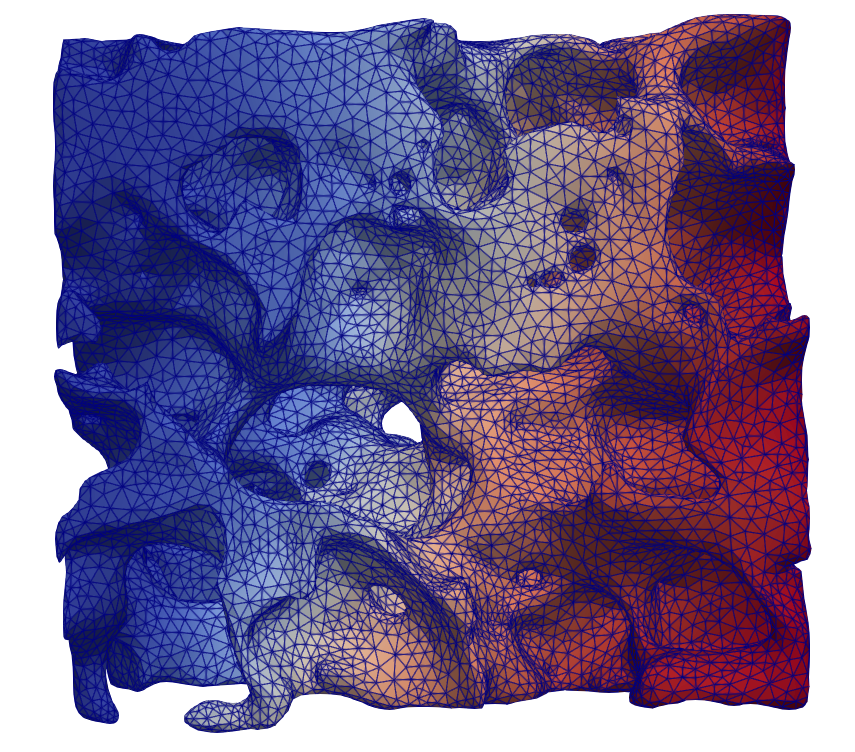
\includegraphics[width=0.45\textwidth]{tum-alveolar-structure.png}

  \caption{Mesh and displacement field of an alveolar structure under axial tension.}
  \label{fig:alveolar-structure}
\end{figure}

\subsection{Heart (POLIMI)}

This section reports on updates on the heart modeling library lifex, which relies on deal.II to build a comprehensive multiphysics tool for the simulation of the cardiac function.

As mentioned in Deliverable 2.1, prior to the start of the dealii-X project lifex relied on conventional matrix-based solvers for all the physical models involved. The solution of linear systems constituted a major bottleneck for performance and parallel scalability \cite{africa2023lifexep,africa2024lifexcfd}, posing a limitation to the scale of problems that could be effectively solved with the library.

Therefore, the POLIMI team is working on migrating the lifex solvers to deal.II's matrix-free infrastructure, and is extensively refactoring the code organization towards this goal. In the new implementation, each concrete PDE model (such as cardiac electrophysiology, muscular mechanics or myocardial perfusion) builds upon the same abstract software components (i.e. is derived from the same classes), as opposed to the old implementation, where different models would often reimplement common tasks (such as the initialization of finite element spaces or linear system assembly). Besides significantly improving the code organization and its maintainability, this centralized structure significantly facilitates the implementation of new physical models and their improvement, and overall provides a structured scaffolding for the future library developments.

The abstract physical model classes at the core of this new implementation leverage deal.II's facilities to support many solver configurations in a flexible way: they allow for scalar- and vector-valued problems, linear and nonlinear, steady and unsteady, on hexahedral and tetrahedral meshes, and support both matrix-based and matrix-free solvers. Finite element evaluation tasks are carried out with the \texttt{dealii::FEEvaluation} class, instead of \texttt{dealii::FEValues} as done in the previous implementation. This enables a significant performance improvement already in the matrix-based solvers, thanks to the use of sum factorization, SIMD vectorization, and to improved cache friendliness.

The solver for the monodomain problem of cardiac electrophysiology has been implemented on top of the new infrastructure, and its parallel performance has been compared to the one of the old code by running a strong scalability test based on the Niederer benchmark \cite{niederer2011verification}. The results (see Figure \ref{fig:lifex-scalability-ep}) show a pronounced improvement in both absolute wall times and parallel scalability, with wall times reduced by a factor 1.5-30, depending on mesh type and number of parallel cores. We note in particular that the vectorization of the ionic solver has lead to a much clearer scalability. This is even more noticeable when observing that the cost of solving ionic models often dominates electrophysiology simulations \cite{africa2023lifexep}.

\begin{figure}
  \centering

  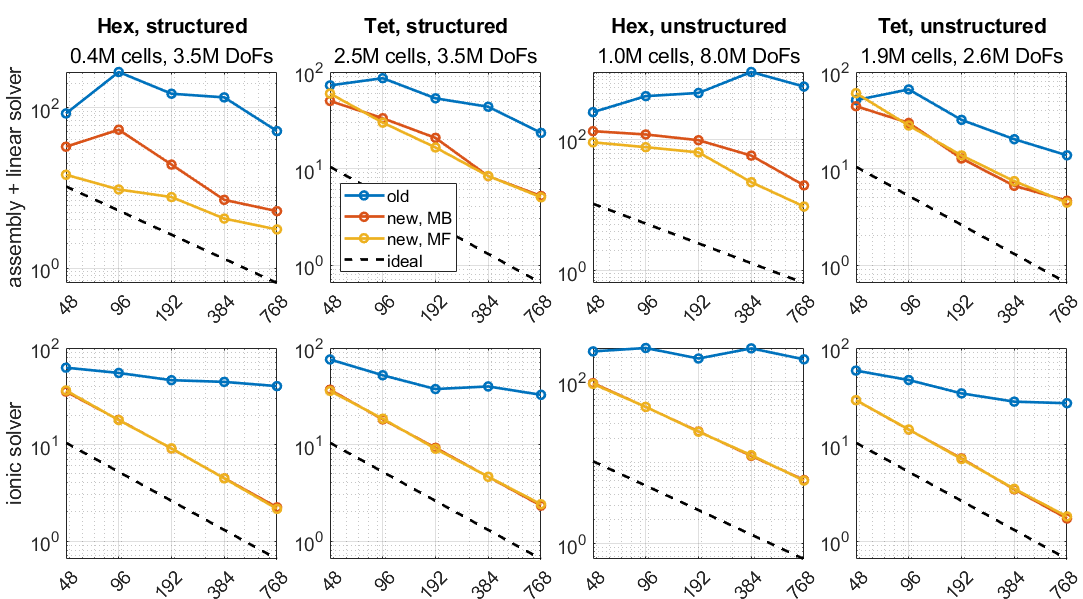
\includegraphics[width=\textwidth]{polimi-lifex-scalability-ep.png}

  \caption{Strong calability of the lifex monodomain solver, in previous (matrix-based) implementation and new (matrix-based and matrix-free) implementation.}
  \label{fig:lifex-scalability-ep}
\end{figure}

Additionally, we have migrated to the new implementation of the multicompartment Darcy solver for myocardial perfusion \cite{zingaro2023comprehensive}, and the solver for generating rule-based cardiac fiber architectures \cite{piersanti2021modeling}. Finally, we are in the process of extending this new framework to the cardiac mechanics solver \cite{fedele2023comprehensive}, as well as coupling the latter to the Darcy model to simulate the behavior of a porous medium subjected to fluid flow.

The upcoming work will follow along these lines, by progressively extending the new infrastructure to additional models (e.g. active force generation for muscular contraction) and introducing coupling between the existing models to build multiphysics simulations (e.g. electromechanics or poromechanics for myocardial perfusion). Complementary to this, we will proceed by expanding the set of numerical methods supported by the core solvers. Most notably, the code currently supports only black-box preconditioning methods (AMG, ILU, etc.), which are not well suited for the matrix-free solvers. Since preconditioning is crucial for the robustness and efficiency of cardiac mechanics solvers, this will be addressed shortly, by integrating a multigrid method within the new code \cite{schussnig2025matrixfree}.

\subsection{Brain (FAU)}

Here, we report on the progress within the ExaBrain library which is developed to facilitate high resolution full human brain finite element simulations using a complex nonlinear poro-viscoelastic material model.

On the one hand, we transferred our code to the National High Performance Computing Center (NHR@FAU) at FAU in Erlangen. This allowed us to perform first benchmarks on the code performance and scalability in an HPC environment which will also serve as the baseline for upcoming developments. Overall, we compared the performance for several system sizes and two different direct solvers. Figure \ref{fig:fau-solver-performance} exemplarily shows the results for the -- so far -- largest system consisting of 24576 hexahedral Q2P1 (quadratic in displacements, linear in pore pressure) elements and 644916 degrees of freedom. The simulations were run on HPC system ``Fritz'' with our baseline parallel direct solver SuperLU-dist and a newly available MUMPS direct solver which was incorporated into deal.II through our project partners at University of Pisa. The new MUMPS solver decreases the memory requirement by approximately \SI{50}{\percent} to \SI{75}{\percent}, depending on the number of parallel processes (Figure \ref{fig:fau-solver-performance}, left). A crucial improvement towards larger systems required for the full human brain. The system assembly does not depend on the solver and scales perfectly with the number of processes (Figure \ref{fig:fau-solver-performance}, middle). While the new MUMPS solver is significantly faster than SuperLU-dist, it does not show good scalability through parallelization (Figure \ref{fig:fau-solver-performance}, right). (The system could not be solved using the SuperLU-dist solver with 64 MPI ranks as this combination exceeded the memory capacity of 256 GB of one compute node at ``Fritz''.)

\begin{figure}
  \centering

  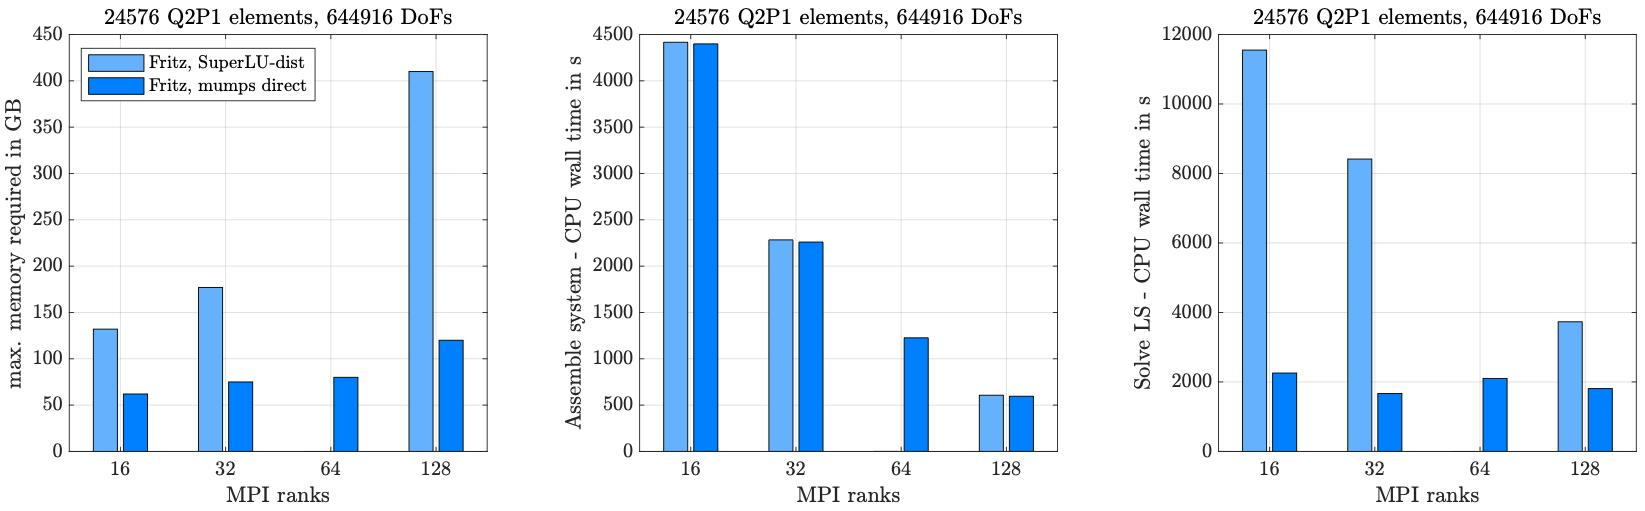
\includegraphics[width=\textwidth]{fau-solver-performance.jpg}

  \caption{Comparison between two parallel direct solvers (SuperLU-dist and MUMPS): memory usage (left), CPU wall time for system assembly (middle) and CPU wall time so solve the linearized system (right).}
  \label{fig:fau-solver-performance}
\end{figure}

Further improvements on the solve phase of the linearized system can be achieved by employing iterative solvers. We report some first comparisons between the direct solvers previously mentioned and GMRES as an iterative solver in Figure \ref{fig:fau-wall-times}. The simulations were run on the University of Pisa HPC system “Toeplitz”. GMRES is preconditioned with the MUMPS solver using the mixed precision Block Low Rank feature. Multiple strategies can be employed to precondition GMRES with BLR: the same preconditioner can be reused to precondition multiple executions of the GMRES solver reducing the number of times the preconditioner has to be evaluated and thus reducing the overall time spent in the linear solver. In Figure \ref{fig:fau-wall-times} we show the differences between evaluating the preconditioner every time we have to solve a linear system (i. e. at each Newton-Raphson step), evaluating the preconditioner once at the beginning of each Newton-Raphson iteration, and updating the preconditioner only if the GMRES iterative solver fails to converge. Ongoing work is focusing on optimizing the number of times the preconditioner must be evaluated in relation to the time required for the convergence of GMRES to further increase the speed of the solve phase.

\begin{figure}
  \centering

  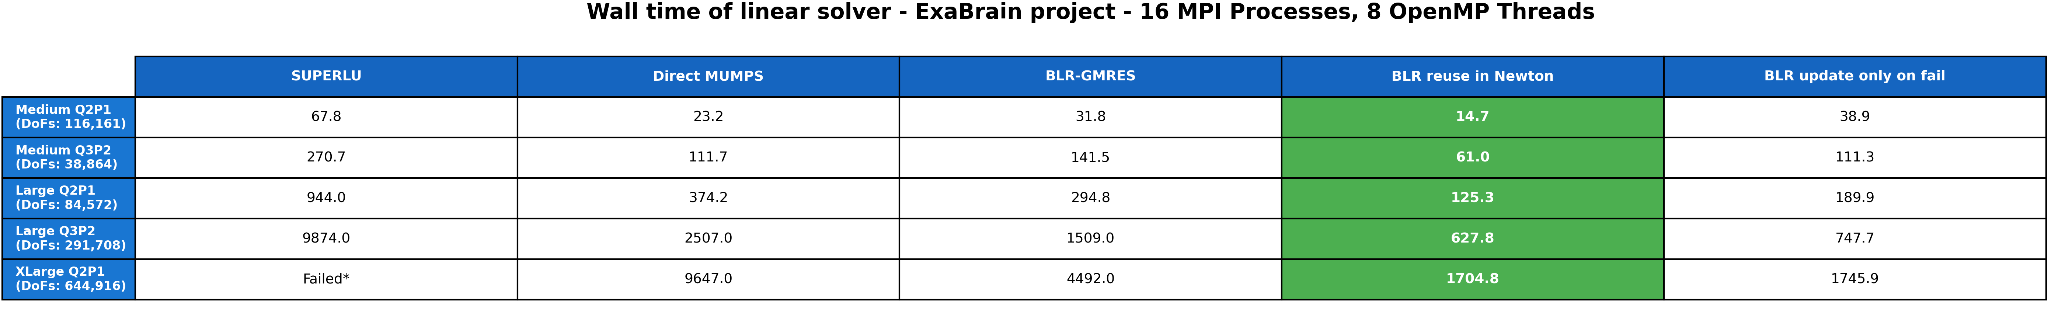
\includegraphics[width=\textwidth]{fau-wall-times.png}

  \caption{Comparison between CPU wall time (s) required by direct and iterative solvers on different sizes of the linear systems solved in a full simulation. SuperLU - dist failed to reach the end of the simulation in the maximum time allowed on the maximum dimension simulation. Each MPI process is using 8 OpenMP Threads.}
  \label{fig:fau-wall-times}
\end{figure}

On the other hand, as full brain simulations require proper material parameters, FAU is working on the efficiency and reliability of the inverse parameter identification. Here, our new HPC possibilities allow us to perform numerical experiments that can then help to identify potential experimental and algorithmic improvements. Figure \ref{fig:fau-inverse-param-identification} shows the results of such a numerical experiment. Starting with a known set of poroelastic parameters ($\mu_\infty = \SI{250}{\pascal}$, $\alpha_\infty = \num{8}$, $K_0 = \SI{1e-8}{\milli\meter\squared}$ and $\lambda^* = \SI{103}{\pascal}$), we performed a relaxation experiment of a cylindrical specimen and evaluated the total nominal stress as well as the lateral displacement of a point on the lateral surface at half of the specimen height (see Figure \ref{fig:fau-inverse-param-identification}a). We then used this numerical ``experimental'' data as an input for our inverse parameter identification with 16 different sets of initial parameters and included once only the total nominal stress into the objective function and once additionally the lateral displacement (equally weighted). Even for this simplified poroelastic example using ``perfect'' experimental data, the nominal stress response alone does not provide enough information to identify a unique parameter set. In fact, only in 12 out of 16 cases we recover the correct parameter set. The situation improves significantly if we incorporate the lateral displacement as additional information (see Figure \ref{fig:fau-inverse-param-identification}b).

\begin{figure}
  \centering

  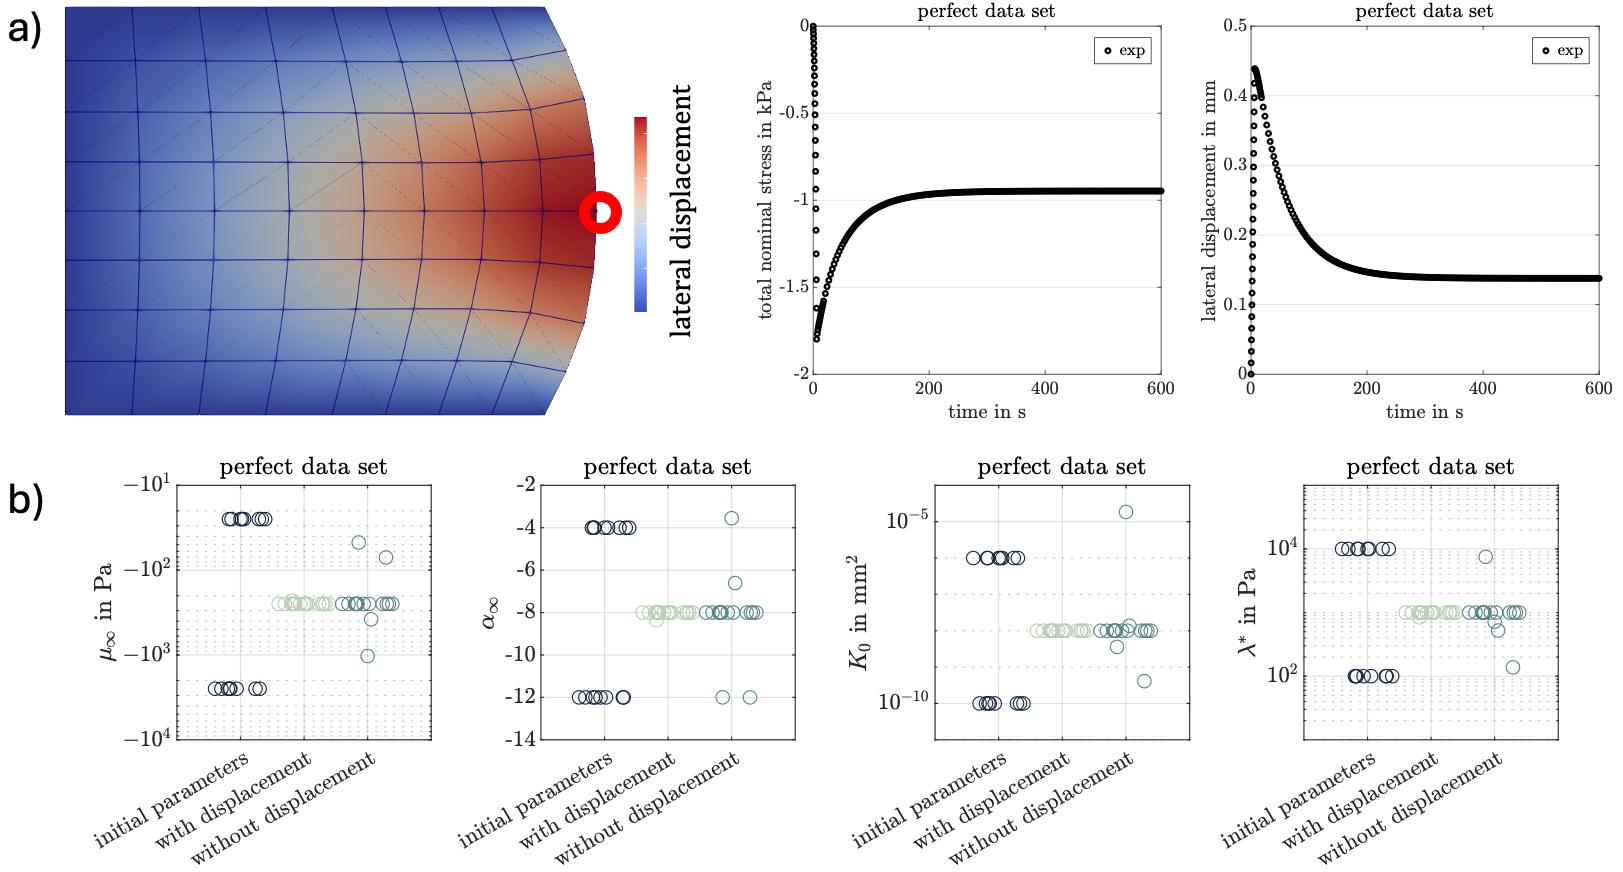
\includegraphics[width=\textwidth]{fau-inverse-param-identification.jpg}

  \caption{Incorporation of additional information (here the lateral displacement) improves reliability of the inverse parameter identification for relaxation tests using a poroelastic material model.}
  \label{fig:fau-inverse-param-identification}
\end{figure}

For our poro-viscoelastic human brain model, the number of unknown model parameters increases from four to seven strongly coupled material parameters. Therefore, numerical experiments as shown in Figure \ref{fig:fau-inverse-param-identification} gain even more importance in understanding the model response and interpreting the results from inverse parameter identifications. With an increasing number of model parameters, we have to cover a significantly larger parameter space where we will benefit substantially from our improvements on the linear solver and the inverse identification itself.

\subsection{Liver (FVB-WIAS)}

This section reports on the liver application. The computational model is built on deal.ii and on the implementation of reduced Lagrange multipliers for multidimensional PDEs. An efficient approach for handling the multiple scales of the problem (fluid flow in the vasculature and elastodynamics in the tissue) is necessary to handle large scale problems.

The reduced Lagrange multipliers approach \cite{heltai2023reduced} formulates the weak coupled (fluid-structure) problem in a weak Lagrange multiplier fashion, applying then a model order reduction based on the properties of the relevant physics (i.e., the approximation that flow can be described by one-dimensional Navier-Stokes equations). The work in WP2.4 focused on the application of this framework to multiscale elasticity.

The reduced Lagrange multiplier  model extends the previous multiscale model proposed in \cite{heltai2019multiscale} to the case of Dirichlet boundary conditions enforced at the vessel-tissue boundaries. This condition is necessary to handle the coupling with pulsatile vasculature. To this purpose, a non-standard interface condition has been considered, which removes macroscopic motion (translational and rotational) and only enforces the coupling at the level of local normal displacement of the vessel. The mathematical framework of \cite{heltai2023reduced} provides the right structure for selecting the proper reduced-order space, and extending these results we proved well-posedness at the continuous level of the new formulation. The model has been used to perform in silico experiments relating the properties of the microstructure to the effective elastic parameters of a tissue sample. These experiments represent the first step towards the formulation of an inverse problem for the parametrization of effective liver samples. Results have been submitted for publication to the International Journal of Numerical Method for Biomedical Engineering.

Following the development of the model, current work is considering the coupling with an active one-dimensional model for the blood flow, extending the previous model of \cite{heltai2021multiscale}. The coupling is implemented representing the one-dimensional network (described by nodes and edges) within the three-dimensional domain as a discrete set of singular points, on which a normal displacement is imposed on the tissue, based on the vessel pulsation. The resulting tissue pressure is, in turn, considered as external force in the blood flow model. The coupling has been first implemented in a staggered fashion, performing preliminary investigations on the stability of the model. A monolithic implementation is under development.

The upcoming work will focus on the generation of realistic vasculatures using physiological parameters specific for the liver, as well as the connection with data assimilation methods to integrate available data for model parametrization.

\subsection{Mechanobiology (UNIBS)}

This section presents recent advancements in mechanobiology, led by the University of Brescia (UNIBS), focusing on the development of advanced computational models to simulate cell motility. Understanding—and ultimately controlling—cell motility is a scientific challenge of the highest order, which underpins metastasis, embryogenesis, and hemostasis. They all rely on non-exiting force-bearing networks, which are purposefully assembled and dismantled in response to physiological demands. Central to this research is the mechanobiological interplay between actin cytoskeleton dynamics and receptor-mediated interactions between the cell membrane and the extracellular matrix. Traditional continuum theories, such as those proposed by Larché and Cahn and Mixture Theories, fall short in capturing the complex coupling of mechanical, chemical, and transport phenomena that govern cytoskeletal reorganization, as they lack the ability to describe the dynamic creation and disassembly of networks. The mathematical foundations of our approach—including the underlying kinematics and balance equations—are detailed in an upcoming publication \cite{salvadori2025chemo}. The computational model is implemented in dealii-X and employs staggered algorithms to solve the coupled PDE system involving chemo-transport and mechanics. Manufactured solutions have been tested in parallel computing environments utilizing multiple processors and distributed memory architectures.

\begin{figure}
  \centering

  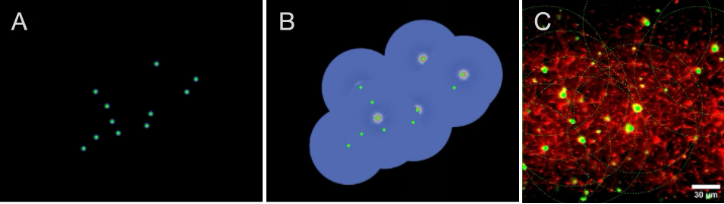
\includegraphics[width=0.75\textwidth]{unibs-load-bearing-networks-1.png}

  \caption{The dealii-X simulation of the formation of load-bearing networks.}
  \label{fig:unibs-load-bearing-networks-1}
\end{figure}

This deliverable focuses on a Lagrangian approach, adopting both global and adaptive local mesh refinement strategies, with the latter guided by the KellyErrorEstimator in deal.II to estimate cell-wise error and improve solution accuracy. Simulations show the ability of the code to generate force-bearing domains upon polymerization of monomers. These simulations apply well in hemostasis, where the growing domain simulates the development of fibrin networks from activated platelets with real data.

\begin{figure}
  \centering

  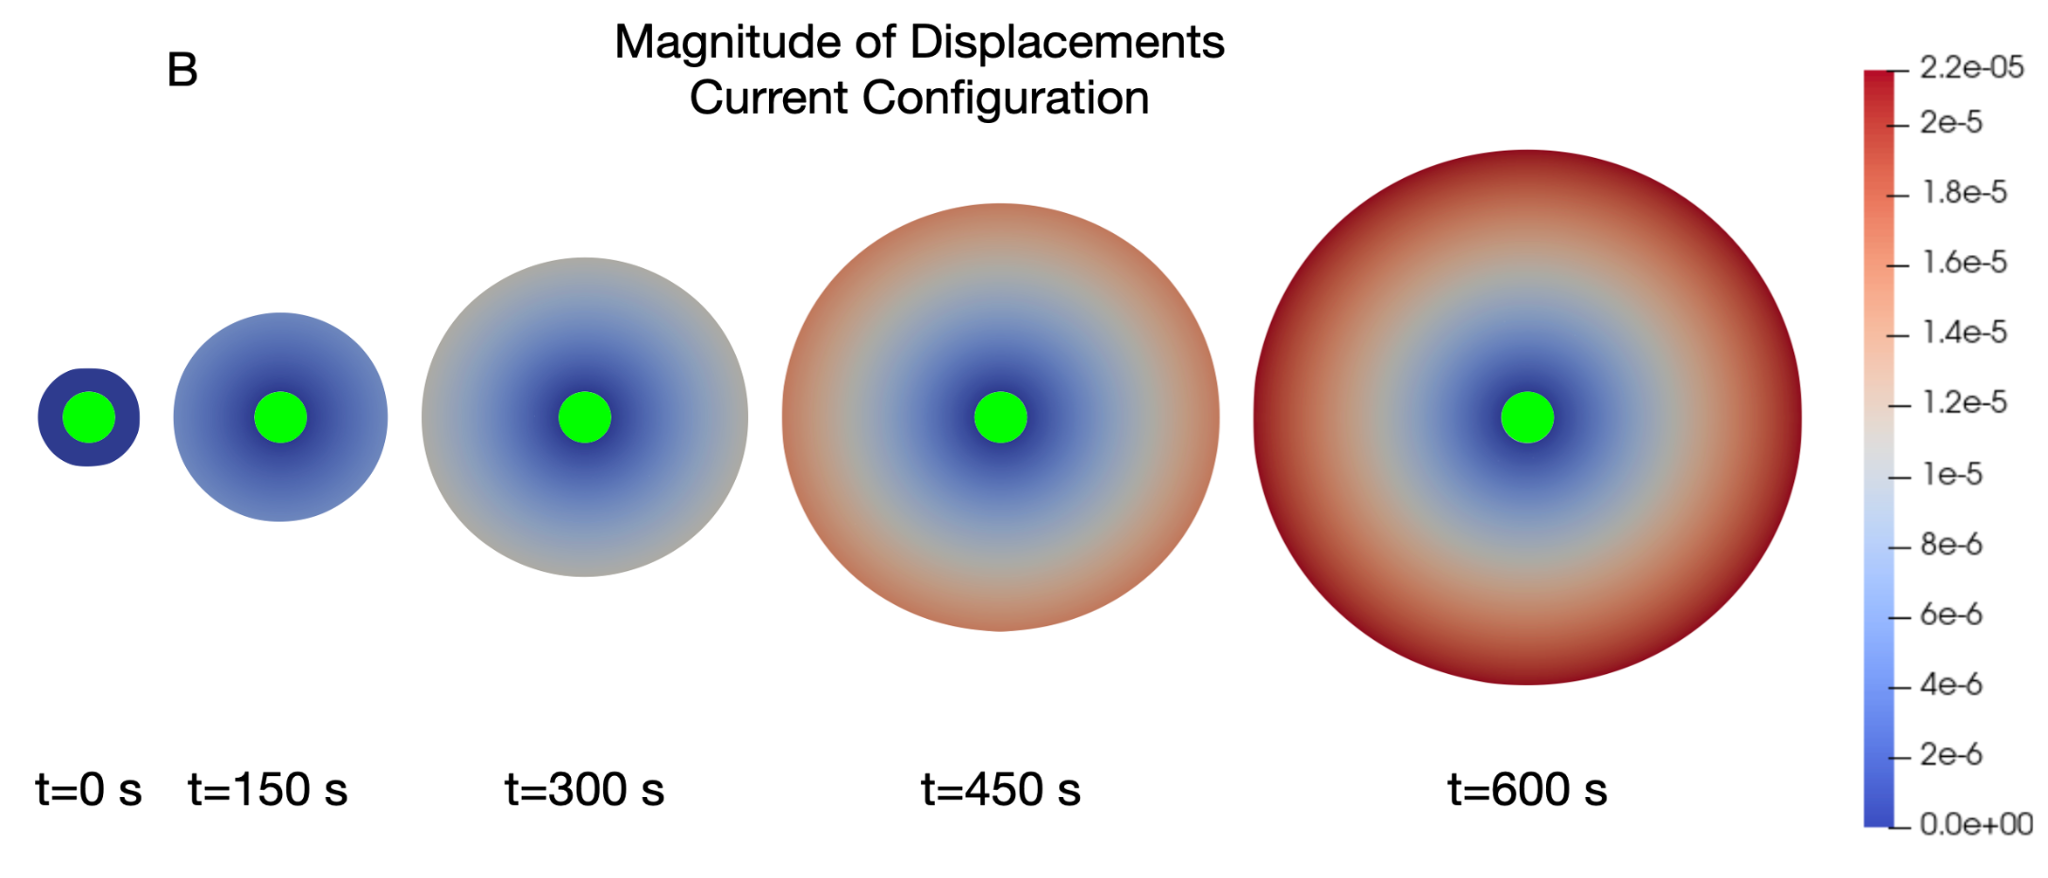
\includegraphics[width=\textwidth]{unibs-load-bearing-networks-2.png}

  \caption{The dealii-X simulation of the formation of load-bearing networks.}
  \label{fig:unibs-load-bearing-networks-2}
\end{figure}

Figure \ref{fig:unibs-load-bearing-networks-1}A shows the initial location of platelets, experimentally identified, surrounded by thrombin that catalyzes the clot formation. Figure \ref{fig:unibs-load-bearing-networks-1}B shows the dealii-X simulation of the load-bearing fibrin network at the end of the simulation, to be compared with the experimental data collected Figure \ref{fig:unibs-load-bearing-networks-1}C. A case study simulation moved from an initial tessellation made of \num{432} quadrilateral elements, distributed across \num{8} processors using parallel memory architectures. Adaptive mesh refinements were applied every \num{150} seconds during a virtual experiment lasting \num{10} minutes. The number of elements increased progressively from \num{432} to \num{6249} by $t = \SI{600}{\second}$, passing through \num{819} ($t = \SI{150}{\second}$), \num{1506} ($t = \SI{300}{\second}$), and \num{3264} ($t = \SI{450}{\second}$). Upon polymerization, the volume of the force-bearing network increases with time. Constraining displacements at the platelet boundary, the volumetric expansion of the fibrin network in the current configuration of the domain at five different time instants ($t = \num{0}, \num{150}, \num{300}, \num{450}$, and $\SI{600}{\second}$) is plotted in Figure \ref{fig:unibs-load-bearing-networks-2}.

The network concentration is reported in Figure \ref{fig:unibs-network-concentration}. Since the activation signal is applied within a fixed region surrounding the platelet in the current configuration, we observe a higher fibrin concentration near the platelet, with decreasing concentrations farther from the activation region.

A Eulerian framework for solids suits well the goal of the dynamic creation and disassembly of networks. The Eulerian perspective is particularly effective in cellular motility, where signaling occurs in localized zones naturally described in the current configuration. Future work will focus on extending the current code, providing realistic mechanisms for the generation and development of the actin cytoskeleton using parameters specific to fibroblasts and potentially other cell types.

\begin{figure}
  \centering

  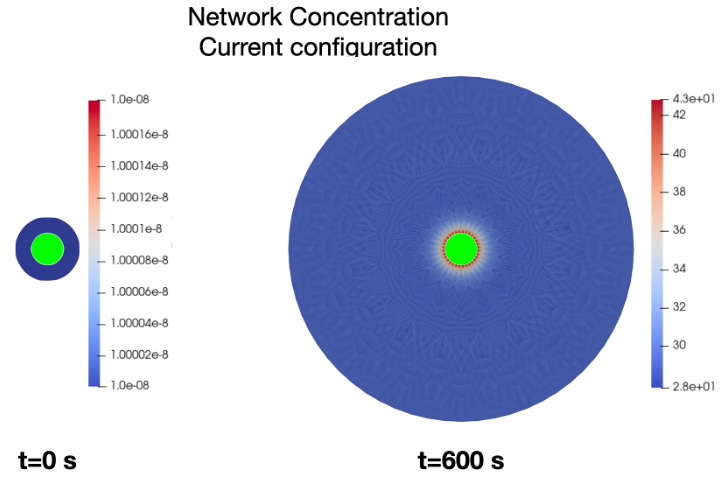
\includegraphics[width=0.75\textwidth]{unibs-network-concentration.png}

  \caption{The dealii-X simulation of the formation of load-bearing networks.}
  \label{fig:unibs-network-concentration}
\end{figure}

\subsection{Dualistic/eXact-Lab}

\subsubsection{Introduction}
The following section reports the progress on the Low-code/No-code interface as well as the related backend. The development follows the approach and the design outlined in deliverable 2.6. The system is composed of three logical parts, which correspond to the following subsections:
\begin{itemize}
  \item \textbf{deal.II-X Client} (Local client app) - the frontend and main user interface, used to create the computation graph and transparently submit calculations;
  \item \textbf{deal.II-X Cloud} (Remote server) - the web server, managing user accounts and communication with the client;
  \item \textbf{CORAL} - the transducer of the computational graph into executable code.
\end{itemize}
The complete architecture is reported in Figure \ref{fig:dualistic-architecture}.

\begin{figure}
  \centering

  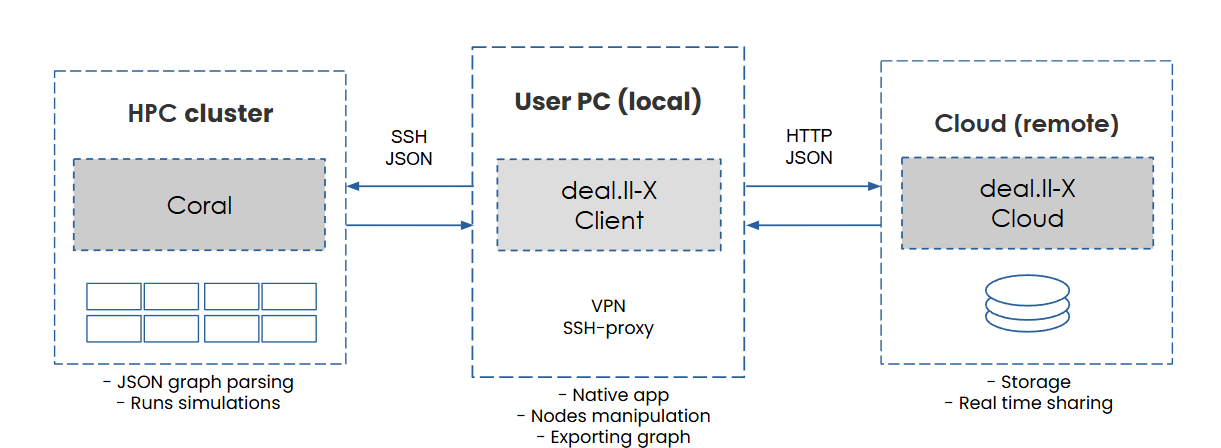
\includegraphics[width=\textwidth]{dualistic-architecture.png}

  \caption{Architecture of the Low-code/No-code interface.}
  \label{fig:dualistic-architecture}
\end{figure}

The client acts as a starting point for every new project. Every new computational graph is created or loaded into the client choosing from a list of available computational nodes. The client will upload each computational graph to the HPC cluster and send the command to start the computation. The state of the computation will be displayed in the client. The client will also save the graph to the remote server and the work will be sharable with other users. The HPC cluster and the cloud will never communicate directly but always throughout the client.

\subsubsection{deal.II-X Client}

The client application provides a no-code graphical interface able to build an editable graph which will then be used to run the simulation in the computing cluster. The graph will be saved and shared among users throughout the remote server. Right now the application is able to import a set of different available nodes and allow the user to draw with them a MWE (Minimal Working Example) that can be exported via SSH secure connection for execution. It can also send simple commands via SSH and send simple HTTP requests. Those features are needed to connect with the computing cluster and with the remote server where Coral will live. The client app is a native cross-platform application running on the user PC. This approach has been chosen over a fully cloud based application, because it provides few key advantages.
\begin{itemize}
  \item Streamlined configuration of the connection to the computing cluster. In particular a direct VPN connection can be established leveraging the connection the user normally uses. SSH configuration is also simplified, with no need for additional tunneling from/to the remote server.
  \item Enhanced security. Users are clearly identified and sensitive data is locally handled, which may be also a requirement for research institutions and other actors.
\end{itemize}

\paragraph{Technologies}
Electron is used to provide native and cross-platform capabilities to the client app. It provides native functionalities from the operating system together with a chromium based environment where any web technology can be used. In particular Svelte and Svelte Flow have been chosen to build the graphical interface, including the canvas from which the graph with nodes and edges is displayed and edited.

Right now a first basic version can be distributed for MacOS and Linux systems or tested in development mode. Core functionalities already available are:
\begin{itemize}
  \item Importing of different basic set of nodes (from a JSON file adhering to a specific protocol)
  \item Exporting the graph via SSH (as a JSON file)
  \item Basic validation on input value and on new edge connection
  \item Basic HTTP requests towards the remote server
  \item Deletion of specific nodes
  \item Drag\&drop of new nodes
  \item Light and dark modes
\end{itemize}

\begin{figure}
  \centering

  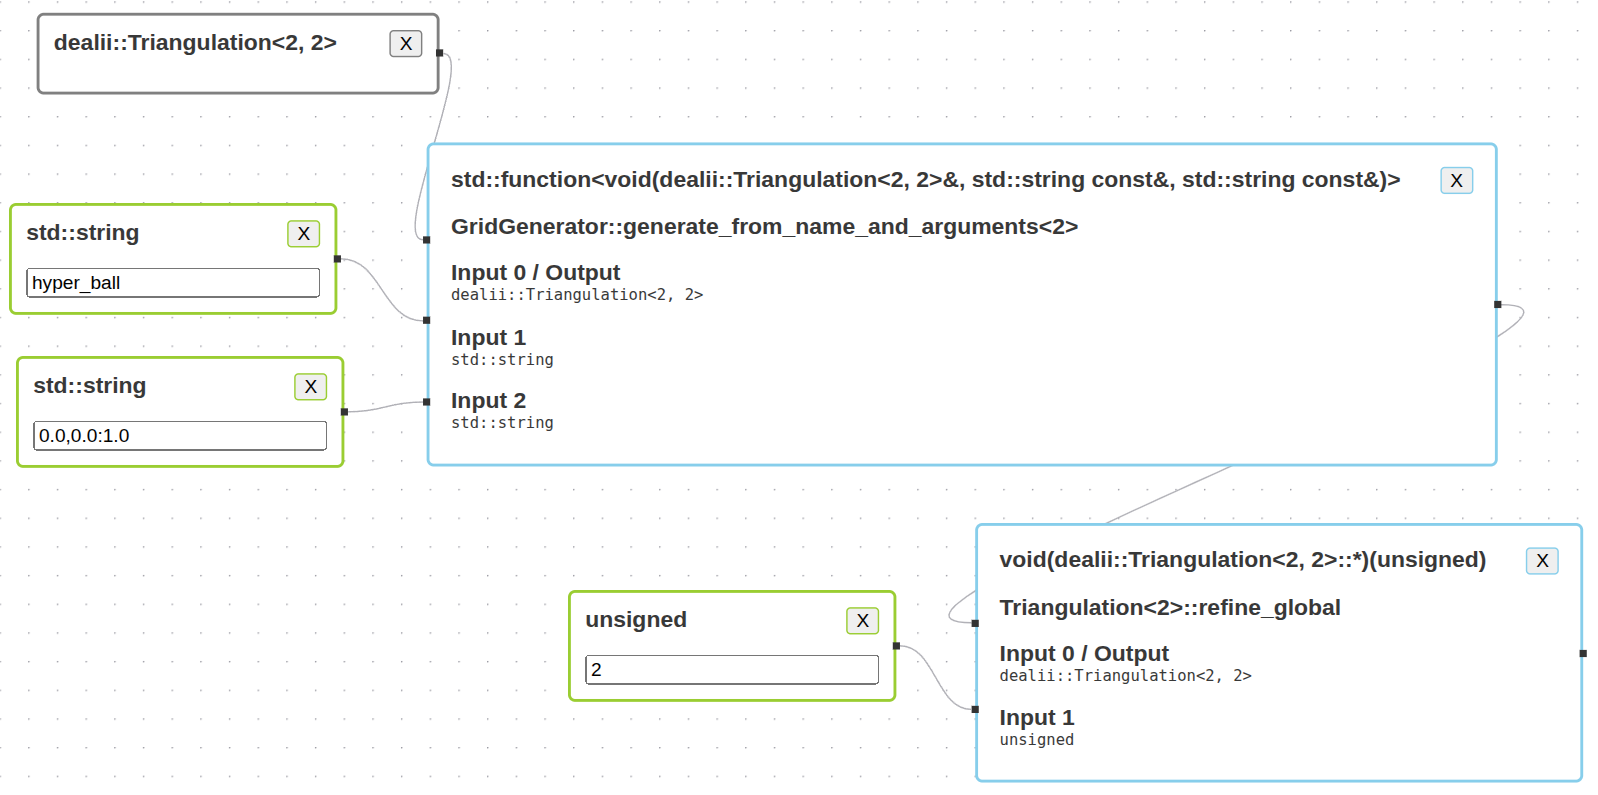
\includegraphics[width=\textwidth]{dualistic-mwe.png}

  \caption{A Minimal Working Example (MWE)  graph in the client app.}
  \label{fig:dualistic-mwe}
\end{figure}

\begin{figure}
  \centering

  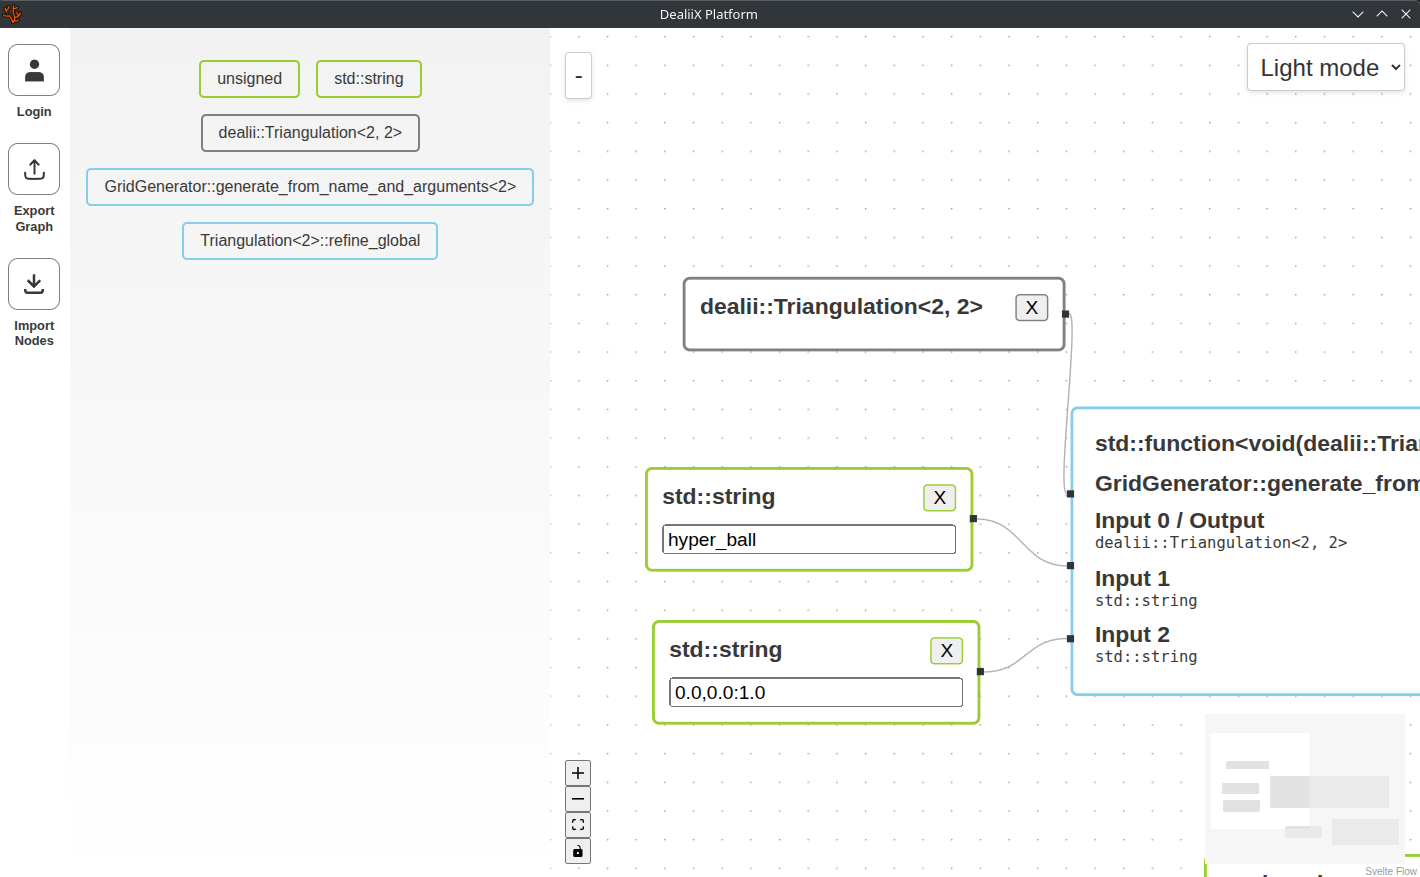
\includegraphics[width=\textwidth]{dualistic-interface-preview.png}

  \caption{A preview of full interface of the client app.}
  \label{fig:dualistic-interface-preview}
\end{figure}

\subsubsection{deal.II-X Cloud}

The deal.II-X Cloud server will be the core of the collaborative nature of the deal.II-X platform, designed to allow sharing of node-based projects between users.  As such, it will sport user authentication, project creation and project sharing. The activities on this component will start in the following months.

\subsubsection{CORAL}

CORAL is a C++ library for building, connecting, and executing computational graphs. It provides a flexible framework for representing computational workflows as directed graphs where nodes represent data or operations, and edges represent dependencies. The library is designed with parallel scientific computing in mind.

In CORAL, every node is designed to be interpreted as a function, represented by its \texttt{operator()}. This functional philosophy ensures that nodes are not merely containers of data or operations but are active participants in the computational graph. The execution of a node's function is determined by its type, which defines its behavior and role within the graph.

In the software stack of the deal.II-X, Coral acts as the transducer of the computational graph generated by the Client application into executable instructions. As such, it runs on the computational infrastructure selected by the user (e.g., an HPC cluster).

The main features of CORAL are:
\begin{itemize}
  \item \textbf{Node as a Function}: each node encapsulates a callable function through its operator(). When invoked, the node performs its designated operation, which may include constructing an object, modifying inputs, or producing outputs.

  \item \textbf{Type-Driven Behavior}: the behavior of a node during execution is controlled by its type. For example:
  \begin{itemize}
    \item \textbf{Constructor Nodes}: these nodes create new objects when executed.
    \item \textbf{Pass-Through Nodes}: these nodes modify their inputs and pass them to their outputs.
    \item \textbf{Method Nodes}: these nodes invoke a specific method on an object, potentially modifying its state or producing a result.
    \item \textbf{Function Nodes}: these nodes execute a free function, using their inputs as arguments and producing outputs.
  \end{itemize}

  \item \textbf{Lazy Evaluation}: nodes are executed only when their outputs are explicitly required by other nodes or the user. This ensures that computations are performed efficiently and only when necessary.

  \item \textbf{Input and Output Management}: each node manages its inputs and outputs through a type-safe system. Inputs are connected to other nodes' outputs, and the execution of the node ensures that the outputs are updated accordingly.
\end{itemize}
This functional approach ensures that nodes in CORAL are versatile and adaptable, capable of representing a wide range of computational tasks. By interpreting nodes as functions, CORAL provides a consistent and intuitive framework for building and executing complex computational workflows.

The core design principles of CORAL are:
\begin{itemize}
  \item Type Safety
  \item Reflection System
  \item Polymorphism Support
  \item Lazy Evaluation
  \item Serialization to JSON
\end{itemize}

The execution model is based on the Taskflow (\url{https://taskflow.github.io/}) library:
\begin{enumerate}
  \item Nodes are registered as tasks in a taskflow graph
  \item Dependencies between tasks are established based on node connections
  \item When execution is requested, tasks are run in the correct order (potentially in parallel)
  \item Results flow through the network as tasks complete
\end{enumerate}
The approach based on graph representation embedded into taskflow allows automatic parallelization of tasks when the graph logically allows it.

\newpage

\section{{Conclusion}} \label{sec:conclusion}

In this document, we have reported the progress made in the digital twin applications of the deal.II-X project.

\bibliographystyle{abbrv}
\bibliography{../common/bibliography.bib}

\label{MyLastPage}

\end{document}
